\section{Experimental Results}
%\lipsum[2]

\subsection{The Dataset}

In our study, we analyze a dataset consisting of historical hourly OHLC (Open, High, Low, Close) data for the eight most liquid crypto exchanges in the market over the recent years. The exchanges chosen for our research are listed in Table \ref{tbl:data}.

\begin{table}[h]
	\centering
	\caption{List of selected exchanges in experimental data-set}
	\begin{tabular}{c|c|c|c}
		Symbol & Distinct Timestamp Count & First Timestamp & Last Timestamp \\
		\hline
		\hline
		ADA/BTC & 25982 & 2022-01-01& 2024-12-18 \\
		BNB/BTC & 25983 & 2022-01-01& 2024-12-18 \\
		BTC/USDT & 25981 & 2022-01-01& 2024-12-18 \\
		DASH/BTC & 25983 & 2022-01-01& 2024-12-18 \\
		EOS/BTC & 25982 & 2022-01-01& 2024-12-18 \\
		ETH/BTC & 25982 & 2022-01-01& 2024-12-18 \\
		LTC/BTC & 25980 & 2022-01-01& 2024-12-18 \\
		XRP/BTC & 25983 & 2022-01-01& 2024-12-18 \\
		
	\end{tabular}
	\label{tbl:data}

\end{table}

Figure \ref{fig:dataset} illustrates the hourly OHLC price histories for the exchanges in the dataset. This dataset provides a comprehensive view of the price movements and trends in the cryptocurrencies market, enabling us to evaluate the performance of the proposed method for stock portfolio management under real-world conditions. 

\begin{figure}[H]
	\centering
	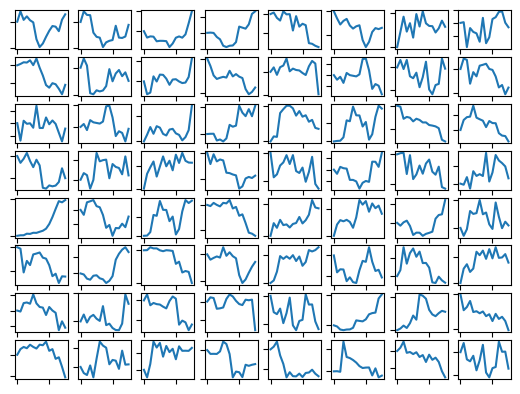
\includegraphics[scale=0.3]{./dataset.png}
	\caption{Illustration of the price series gathered in the dataset.}
	\label{fig:dataset}
\end{figure}



In the rest of this section we will investigate different aspects of the proposed model in portfolio management. Section 4.2 studies the features of the latent space learned by the VAE model. Section 4.3 provides an ablation study on the proposed model and a makes a comparison between the different versions of the proposed model. Section 4.4 compares the results of the proposed model with the baseline models.

\subsection{Latent Space Investigation}
In this experiment, we explored the latent space of a Variational Autoencoder (VAE) trained on time-series data. The model was designed to disentangle the input space into two distinct latent representations: one capturing the trend of the price series and the other representing the variance. To facilitate a focused analysis, the dimensionality of both the trend and variance variables was constrained to one. This simplification allowed for a straightforward visualization and interpretation of the latent space.

The encoder of the VAE outputs two latent variables, denoted as $\mu$ (mean) and $\sigma^2$ (variance), corresponding to the trend and variance representations. By iterating over the $\mu$-$\sigma^2$ space, we sampled time-series data using the decoder. These generated series were visualized in a 2D graph, where each point in the $\mu$-$\sigma^2$ grid corresponds to a generated time-series. The resulting graph contains 64 generated images arranged systematically across the latent space, divided into four distinct sub-spaces for analysis.

Figure \ref{fig:latent_full} demonstrates a 2D visualization as a comprehensive view of the latent space and its impact on the generated time-series. The graph is structured into four sub-spaces, with notable differences in the nature of the generated series:

\begin{enumerate}
	\item Upper sub-spaces:
	The generated series in the upper half of the latent space resembles the mathematical function $sin(x)$ for the range $-\frac{\pi}{2} < x < \frac{\pi}{2}$. These series exhibit smooth oscillations and a consistent periodicity, suggesting that the upper latent sub-spaces predominantly capture sinusoidal positive price trend.
	
	\item Lower sub-spaces:
	In the lower half of the latent space, the generated series align more closely with $sin(x)$ for the range $0 < x < \frac{\pi}{2}$. These series exhibit similar periodic behavior but with a phase shift compared to the upper sub-spaces, indicating a separation in phase dynamics within the latent representation.
	
\end{enumerate}

The primary contribution of this illustration is showcasing the VAE's ability to decompose price series into small wave-like patterns resembling sinusoidal functions in various phases. This indicates the model's capability to detect trend shifts effectively. By inputting a test time-series at each timestep, the VAE maps the historical price data into its trained latent space. The latent space then associates the input series with specific sub-spaces defined by the corresponding $\mu$ and $\sigma^2$ values.

\begin{figure}[h]
	\centering
	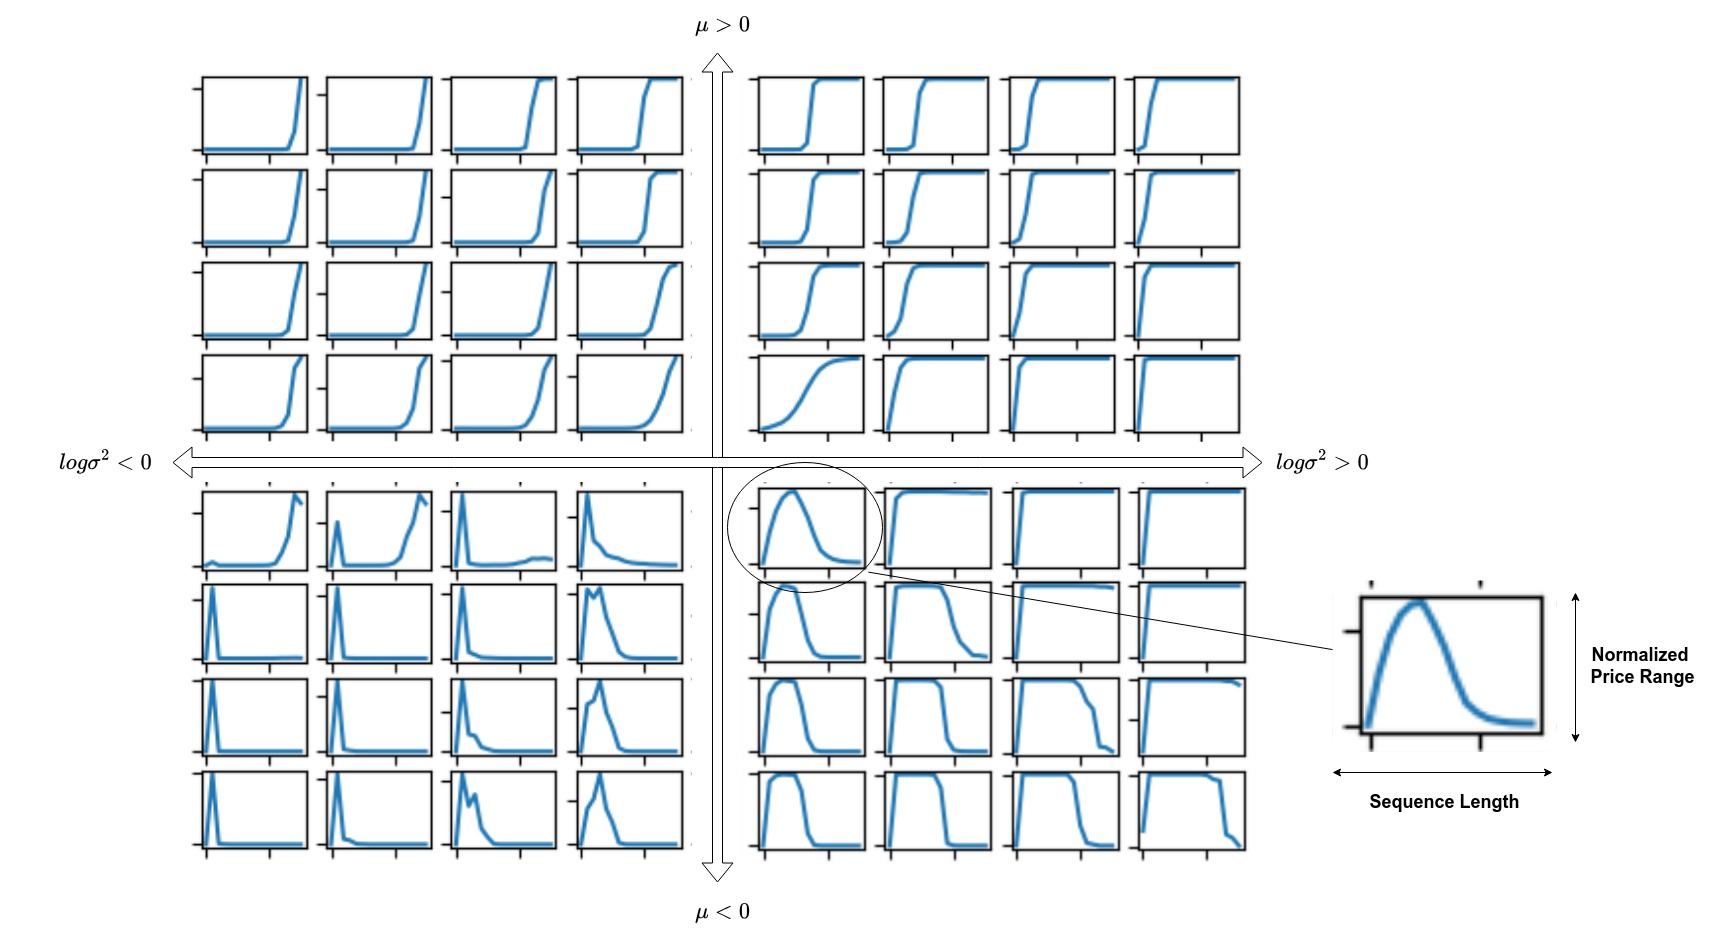
\includegraphics[scale=0.25]{./LatentSpace.jpg}
	\caption{Illustration of the latent space learned by VAE with classifier over model performance series}
	\label{fig:latent_full}
\end{figure}


\subsection{Ablation Study}

To assess the effectiveness of different components of the proposed method, we conduct an ablation study where we systematically analyze the impact of key elements such as the VAE for uncertainty measurement and the Actor-Critic neural network for stock portfolio proposal. By comparing the performance of the complete model with variations that exclude specific components, we aim to understand the contribution of each part to the overall coin switching strategy.

\subsubsection{Feature Extraction}
In the initial experiment in ablation study, our objective is to examine the influence of the VAE model on classification of price trend movement direction. For this aim, we utilize a multi-layer perceptron (MLP) network to categorize the direction of price movements based on the definition outlined in equation \eqref{eq:class1}. The outcomes of price trend prediction using various classifiers are compared in Table \ref{tbl:FE-pred}.

The baseline models considered in this study are as follows:
\begin{itemize}
	\item \textbf{MLP}. This model is a basic MLP classifier trained directly on the input series without any feature extraction.
	\item \textbf{VAE-Z}. Here, the VAE is trained, and only the embedding vector $Z$ is provided to the classifier as the extracted feature.
	\item \textbf{VAE-TR}. In this model, the VAE is trained, and the concatenated latent vectors $\hat{\mu}$ and $\hat{\sigma}$ are passed to the classifier as the extracted feature.
	\item \textbf{VAE-Y}. This model involves training the VAE, and only the VAE's embedded classifier output $\hat{Y} = \Phi(\hat{\mu}, \hat{\sigma})$ is used as the extracted feature.
	\item \textbf{VAE-FULL}. In this setup, the VAE is trained, and all encoder outputs containing $Z$, $\hat{\mu}$, and $\hat{\sigma}$ are concatenated and provided to the classifier as the extracted feature.
\end{itemize}

Table \ref{tbl:FE-pred} presents a comparison of the baseline models' accuracy in the classification task. The results indicate that model \textbf{VAE-Y} performs the best as a feature extractor. This observation supports our hypothesis that accurately predicting the likelihood of continuation of the current stock price trend can assist portfolio management models in determining optimal points for asset switching within the portfolio.

\begin{table}[h]
	\centering
	\caption{Comparison between baseline models accuracy in predicting the future price trend direction}
	\label{tbl:FE-pred}
	\begin{tabular}{c | c | c | c | c | c }
		Method & MLP & VAE-Z & VAE-TR & VAE-Y & VAE-FULL \\
		\hline
		\hline
		Train & 63.48& 76.94 & 95.36 & \textbf{95.45} & 94.36\\
		Test & 61.80& 73.59 & 93.47 & \textbf{95.55} & 94.72\\
	\end{tabular}
\end{table}

\subsubsection{Latent Space Dimensionality}
The following experiment aims to explore how the size of latent vectors $\hat{\mu}$ and $\hat{\sigma}$ influences the quality of extracted features. In this study, we varied the dimensions of the latent vectors and assessed the classifier's accuracy in predicting the next price movement direction.

The comparison of these models is presented in Table \ref{tbl:FE-dim}. The findings from this table suggest that enhancing the dimensionality of latent vectors leads to improved model performance. This improvement can be attributed to the larger latent vector size enabling the model to more effectively encapsulate the extracted information into a single vector. It is worth noting that as the dimensionality increases, more data is required for training, and therefore, performance gains may plateau after reaching a certain threshold with a fixed dataset size.


\begin{table}[h]
	\centering
	\caption{The impact of the latent vectors size on the accuracy of the price trend prediction}
	\label{tbl:FE-dim}
	\begin{tabular}{c | c | c | c | c | c }
		Method & 1 & 10 & 50 & 150 & 200 \\
		\hline
		\hline
		Train & 95.45& 96.02 & 98.51 & \textbf{98.85} & 95.46\\
		Test & 95.55& 94.16 & 97.37 & \textbf{98.23} & 91.24\\
	\end{tabular}
\end{table}

\subsubsection{Reward Function}
The reward function proposed for the coin-switching agent in equation \ref{eq:ri} is designed based on the distance between the selected coin by the agent and the best coin at each time step. This approach aims to give incentive to the agent to learn to switch to the best coin at every time step. Another commonly used reward function in this research domain is the total portfolio return at each time step. To evaluate the effectiveness of the proposed reward function, a comparison between these two models is presented in table \ref{tbl:rewards}. The table includes metrics such as total return on investment (\textbf{total-ROI}), maximum drawdown (\textbf{MDD}), and average return (\textbf{AR}) for each model. The results indicate that the model utilizing the proposed return function demonstrates superior performance compared to the traditional reward function commonly used in the field.


\begin{table}[h]
	\centering
	\caption{The impact of proposed reward function}
	\label{tbl:rewards}
	\begin{tabular}{c | c | c | c  }
		Method & total-ROI & MDD & AR \\
		\hline
		\hline
		Proposed Reward & \textbf{125 \%}  & \textbf{-19 \%} & \textbf{0.27}  \% \\
		Common Reward & 54 \%  & -20 \%  & 0.15 \%\\
	\end{tabular}
\end{table}

%
%\subsubsection{Considering Risk-free Asset}
%One of the main underlying assumptions in our study was that mitigating minor losses would enhance portfolio management effectiveness. Consequently, we conducted an additional experiment to investigate how our model performs with and without the inclusion of a risk-free asset. Table \ref{tbl:rf1} presents a comparison of the model's performance under these conditions. The results indicate that the model performs better when the risk-free asset is included, particularly in terms of metrics such as maximum drawdown. This suggests that timely switching to the risk-free asset can help prevent losses in the investment process.
%
%\begin{table}[h]
%	\centering
%	\caption{The impact of risk-free asset presence on model's performance}
%	\label{tbl:rf1}
%	\begin{tabular}{c | c | c | c  }
%		Method & total-ROI & MDD & AR \\
%		\hline
%		\hline
%		with tether & \textbf{125 \%}  & \textbf{-19 \%} & \textbf{0.27}  \% \\
%		without tether & 28 \% & -34 \% & 0.11 \% \\
%	\end{tabular}
%\end{table}

%To demonstrate the efficiency of the proposed model in identifying and transitioning to the risk-free asset at opportune moments, we conducted an additional experiment. In this study, we defined periods where all coins exhibited a bearish price trend as bearish markets, with all other times classified as bullish. Subsequently, we evaluated the behavior of the coin-switching agent in terms of its ability to switch to the risk-free asset during bearish market conditions. The outcomes of this experiment are presented in Table \ref{tbl:rf2}. The true positive metric (TP) signifies the percentage of instances where the coin-switching agent correctly switched to the risk-free asset, while the false positive metric (FP) indicates the percentage of incorrect switches, and so forth. The results reveal that in the presence of a risk-free asset, the model effectively learns to transition to this asset when the majority of other coins are experiencing a bearish price trend. Our findings demonstrate that the coin-switching agent successfully switched to the risk-free asset in approximately 30\% of instances when all available coins were in a bearish trend.
%
%\begin{table}[h]
%	\centering
%	\caption{The confusion matrix of the proposed model indicating the power of the model in switching to the risk-free asset at proper times.}
%	\label{tbl:rf2}
%	\begin{tabular}{c | c | c }
%		Market & Positive & Negative \\
%		\hline
%		\hline
%		Positive & 0& 0 \\
%		Negative & 0& 0 \\
%	\end{tabular}
%\end{table}

%The experiment's results is summarized to compare various iterations of the proposed model. Table \ref{tbl:cmp1} presents the performance metrics of these models for comparison. The findings from the table indicate that the model utilizing \textbf{VAE-Y} as the feature extractor and incorporating the suggested reward function that accounts for the risk-free asset outperforms other versions of the model.

\subsection{Portfolio Proposals}
The primary objective of the proposed model is to identify optimal time points for transitioning between different coins in the market. While the model's primary focus is distinct from portfolio management in which models are supposed to propose a combination of instruments at each time-step, we conducted a performance evaluation by comparing it against both single asset trading strategies and portfolio management models to assess its effectiveness in identifying optimal transition points between coins.

\subsubsection{Baselines}
The baseline models that have been compared with the proposed model are outlined below:

\begin{itemize}
	\item \textbf{BaH(X)}(\citet{li2014online}). This denotes the buy and hold strategy, where coin X is purchased at the beginning of the experiment and held until the end.
%	\item \textbf{MLP-vanilla} \citet{taghian2022learning}.  This model, introduced by \citet{taghian2022learning}, involves a Deep Reinforcement Learning (DRL) model that learns candlestick patterns and establishes generalized trading rules for Bitcoin.
	\item \textbf{UCRP}(\citet{li2014online}). Uniform Constant Rebalanced Portfolio strategy involves setting the portfolio proposal vector to a uniform vector $w^t=(\frac{1}{n}, \cdots, \frac{1}{n})$ at the start of each time step, where $n$ represents the number of available coins and $|w^t| = n$.	
	\item \textbf{FTW}. Following the winner strategy adjusts the portfolio proposal vector at each time step based on the historical performance of coins, with weights of winning coins revised according to their cumulative return $w^t = SoftMax(CR_t)$, where $CR_t$ is calculated as in equation \eqref{eq:ftw}.
	\begin{align}
		CR_t = \{R(X_i^{1:t})| \> &X_i^{1:t} = \{X_i^1, \cdots, X_i^t\} \> \land  \notag \\ 
		&R(X_i^{1:t}) = \frac{X_i^t}{X_i^1} \> \land \notag \\ 
		&i \in \{1, \cdots, n\}\}
		\label{eq:ftw}
	\end{align}

	\item \textbf{FTL}. Following the loser strategy refines the portfolio proposal vector at the beginning of each time step by adjusting the weights of losing coins based on the inverse of their historical performance $w^t = SoftMax(CR_t^{-1})$, using $CR_t^{-1}$ computed as shown in equation \eqref{eq:ftl}.
	\begin{align}
	CR_t^{-1} = \{R(X_i^{1:t})^{-1} | &X_i^{1:t} = \{X_i^1, \cdots, X_i^t\} \> \land \notag\\ 
	&R(X_i^{1:t})^{-1} = \frac{1}{1 + log(\frac{X_i^t}{X_i^1})} \> \land \notag \\  
	&i \in \{1, \cdots, n\} \}
	\label{eq:ftl}
	\end{align}
\end{itemize}

\subsubsection{Deep Learning Models}
The state-of-the-art models that have been compared with the proposed model are outlined below:

\begin{itemize}
	\item \textbf{LSTM-GARCH}(\citet{garcia2024lstm}). This approach employs a GARCH model to estimate the variance of each price series. The resulting variance estimates are then input into an LSTM network to generate portfolio vectors at each timestep.
	
	\item \textbf{Transformer}(\citet{kumar2024transformer}). This model utilizes a Transformer network for price prediction, integrated with a DQN framework for decision-making.
	
\end{itemize}

For all the models discussed above, we implemented the proposed architectures as described in the original papers and conducted evaluations using our dataset to ensure consistency and reproducibility of the results.


\subsubsection{Comparison results}

Table \ref{tbl:cmp} presents the comparison of the performance of the proposed model against the baseline models in terms of total return on investment (RoI), maximum drawdown, and average return. In this table, the term $CoinSwitching$ denotes the proposed model with the common reward term, while $CoinSwitching^*$ represents the proposed model with the proposed reward function, which is considered the most effective version of the proposed model.

\begin{table}[h]
	\centering
	\caption{Comparison of the performance of the proposed model versus portfolio management, and single asset trading strategies.}
	\label{tbl:cmp}
	\begin{tabular}{l| c | c | c | c | c | c  }
		Strategy & Model & total-ROI & MDD & AR & Accuracy & Hit Rate\\
		\hline
		\hline
		\multirow{5}{*}{Single-Asset} 	& BaH(ETH/BTC) & -17.18 \%  & -20 \% & 0.17 \% & 13.26 \% & 39.98 \% \\
										& BaH(BTC/USDT) & 0.32 \%  & -27 \% & 0.08  \% & 11.08 \% & 48.56 \% \\
										& BaH(BNB/BTC) & -2.33 \%  & -41 \% & 0.06  \% & 18.51 \% & 50.66 \% \\
										& BaH(XRP/BTC) & -14.74 \%  & -73 \% & 0.21 \% & 14.16 \% & 40.60 \% \\
										& BaH(LTC/BTC) & -34.34 \%  & -59 \% & 0.13  \% & 12.89 \% & 41.01 \% \\
										& BaH(ADA/BTC) & -8.30 \%  & -59 \% & 0.13  \% & 5.91 \% & 44.99 \% \\
										& BaH(DASH/BTC) & -13.98 \%  & -59 \% & 0.13  \% & 12.11 \% & 42.86 \% \\
										& BaH(EOS/BTC) & -11.93 \%  & -59 \% & 0.13  \% & 12.07 \% & 40.93 \% \\
%										& MLP-vanilla \citet{taghian2022learning} & 248506 \%  & -82 \% & 1.87  \% \\
		\hline
		\hline
		\multirow{3}{*}{Baselines} 	& UCRP & -6.76 \%  & -35 \% & 0.010 \% & 13.26 \% & 39.98 \% \\
												& FTW & -73.86 \%  & -33 \% & 0.017  \% & 12.52 \% & 37.93 \% \\
												& FTL & -68.43 \%  & -41 \% & 0.014  \% & 11.45 \% & 40.85 \% \\
		\hline
		\hline
		\multirow{2}{*}{Deep Models} 	& LSTM-GARCH & -31.81 \%  & -46 \% & 0.13 \% & 15.15 \% & 44.58 \% \\
									& Transformer & -22.14 \%  & -3.38 \% & 0.16  \% & 14.82 \% & 45.03 \% \\
		\hline
		\hline
		\multirow{2}{*}{Proposed Model}  	& $CoinSwitching$ &  54.1 \%  & -20 \%  & 0.15 \%& 15.89 \% & 43.96 \% \\
											& $CoinSwitching^*$ & \textbf{163.41 \%}  & \textbf{-19 \%} & \textbf{0.27}  \% & 16.38 \% & 48.07 \% \\
	\end{tabular}
\end{table}

Furthermore, the diagram in Figure \ref{fig:versions} illustrates the evolution of portfolio values for various strategies over time. It is evident from the graph that the suggested approach outperforms other strategies by mitigating minor losses. While different segments of the proposed strategy's portfolio value curve resemble those of other strategies, the key distinction lies in its ability to avert losses by switching between selected coins, thereby enhancing overall portfolio performance significantly.

\begin{figure}[h]
	\centering
	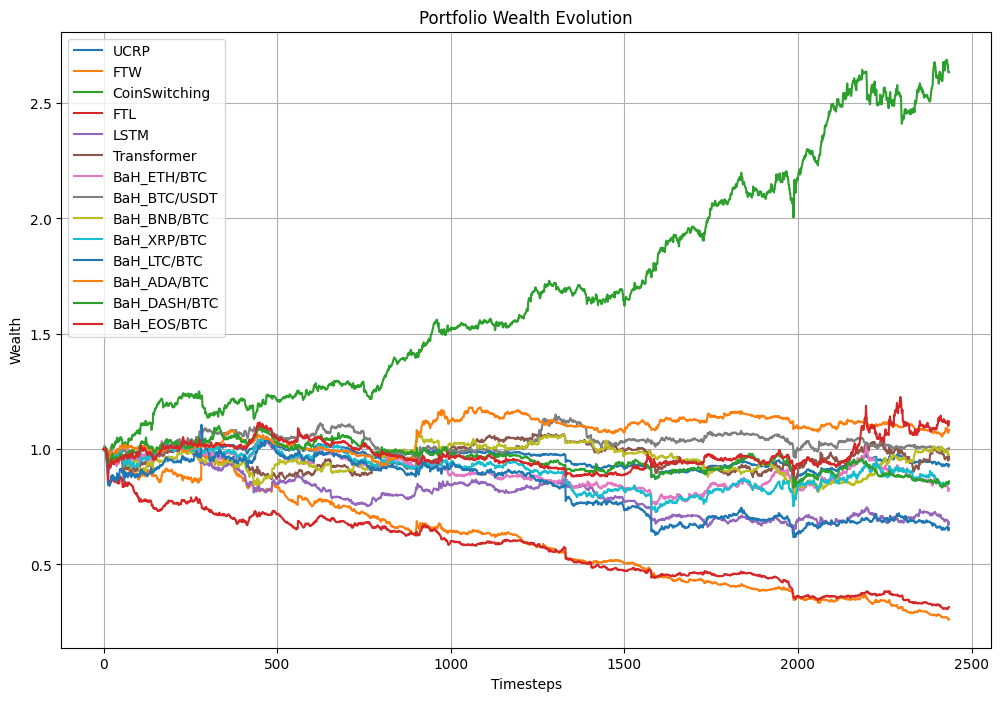
\includegraphics[scale=0.6]{./ms1.png}
	\caption{Comparison of the proposed model with single asset strategies.}
	\label{fig:versions}
\end{figure}

Moreover, Figure \ref{fig:changes1} depicts the behaviors of the optimal coin-switching strategy over the investment period. As shown in the figure, the strategy predominantly involves switching between coins when there are noticeable declines in coin prices, while minor price fluctuations have minimal impact on the agent's decisions.



\begin{figure}[h]
	\centering
	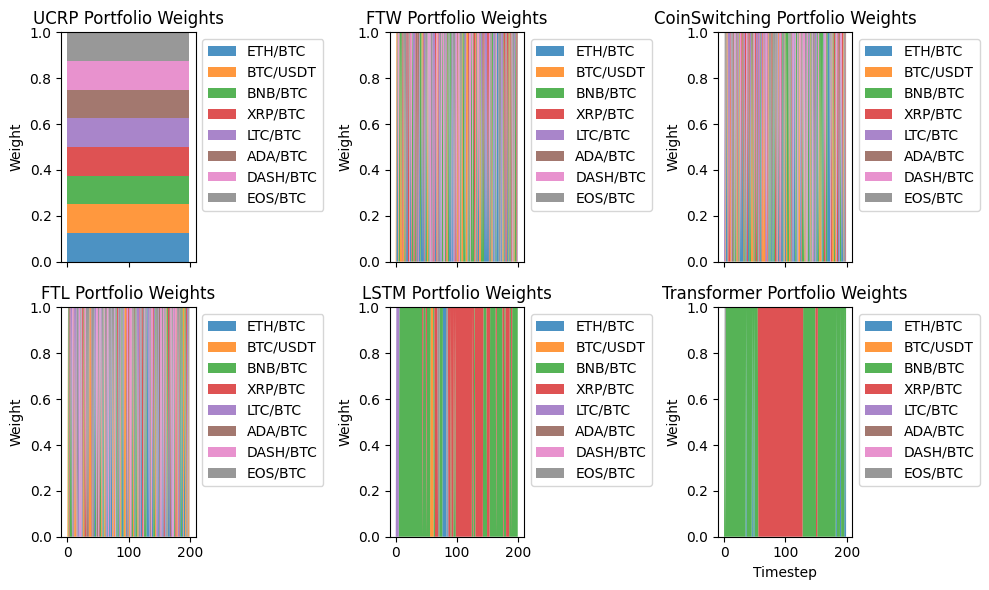
\includegraphics[scale=0.6]{./changes1.png}
	\caption{Model selection during investment timesteps}
	\label{fig:changes1}
\end{figure}

